\documentclass[UTF8,a4paper,12pt,fontset=fandol]{ctexart}

\usepackage{geometry}
\usepackage{graphicx}
\usepackage{float}
\usepackage{booktabs}
\usepackage{array}
\usepackage{xcolor}
\usepackage{listings}
\usepackage{hyperref}

\geometry{left=2.5cm,right=2.5cm,top=2.5cm,bottom=2.5cm}
\hypersetup{colorlinks=true,linkcolor=black,urlcolor=blue}

\lstset{
  basicstyle=\ttfamily\small,
  breaklines=true,
  frame=single,
  columns=fullflexible,
  keepspaces=true,
  backgroundcolor=\color{gray!8}
}

\title{基于 Jetson、YOLO 与 ROS2 的桌面目标实时检测实验报告}
\author{姓名：\underline{\hspace{4cm}} \quad 学号：\underline{\hspace{4cm}}}
\date{\today}

\begin{document}

\maketitle

\begin{abstract}
本实验面向桌面场景中的常见物体检测任务，完成了数据采集、数据标注、YOLO 模型训练、Jetson 开发板部署以及 ROS2 实时结果发布。实验最终采用 YOLOv8s 预训练权重进行迁移训练，检测类别为 cup 和 mouse，并在 Jetson 平台上通过摄像头进行实时识别。为满足机器人系统通信需求，实验将检测程序封装为 ROS2 节点，实时发布检测结果 topic，使其他 ROS2 节点能够订阅目标类别、置信度和检测框坐标。实验结果表明，该方案能够在 Jetson 上达到课程要求的实时检测帧率，并能够完成桌面杯子和鼠标的实时识别。
\end{abstract}

\section{实验目的}

本实验的主要目标如下：

\begin{enumerate}
  \item 掌握目标检测数据集的采集、标注与 YOLO 格式组织方法；
  \item 使用 YOLO 预训练模型完成桌面目标检测模型训练；
  \item 将训练完成的模型部署到 NVIDIA Jetson 开发板；
  \item 使用摄像头完成实时目标检测，并显示类别、检测框和置信度；
  \item 使用 ROS2 发布检测结果，使检测模块能够接入机器人软件系统。
\end{enumerate}

\section{实验环境}

\begin{table}[H]
\centering
\begin{tabular}{>{\raggedright\arraybackslash}p{4cm}p{9cm}}
\toprule
项目 & 配置 \\
\midrule
训练平台 & macOS，Apple M3，CPU 训练 \\
部署平台 & NVIDIA Jetson，Ubuntu 22.04.5 LTS，aarch64 \\
开发语言 & Python \\
深度学习框架 & Ultralytics YOLO，PyTorch \\
图像处理 & OpenCV \\
机器人通信 & ROS2 \\
模型版本 & YOLOv8s 迁移训练模型，最终部署版本为 v4 \\
检测类别 & cup，mouse \\
\bottomrule
\end{tabular}
\caption{实验软硬件环境}
\end{table}

\section{数据集构建}

本实验使用 Roboflow 对桌面物体图片进行手动标注，并导出 YOLO 目标检测格式数据集。YOLO 标签文件中每一行表示一个目标，格式为类别编号、中心点坐标、检测框宽度和检测框高度，坐标均为相对于图像尺寸的归一化数值。

本实验最终用于 YOLOv8s v4 训练和 Jetson 演示的主要类别为 cup 和 mouse。数据集中还整理过 bottle 类数据，用于后续扩展，但最终 Jetson 演示模型仍采用 cup 与 mouse 两类模型，避免由于 bottle 样本较少导致实时演示不稳定。

\begin{table}[H]
\centering
\begin{tabular}{lc}
\toprule
数据划分 & 图像数量 \\
\midrule
训练集 & 959 \\
验证集 & 183 \\
测试集 & 58 \\
\bottomrule
\end{tabular}
\caption{合并后的数据集规模}
\end{table}

在真实桌面场景测试中，模型曾出现复杂背景下的误检和漏检。例如玻璃杯、水壶、鼠标垫纹理、衣物和人脸背景可能影响检测结果。因此实验过程中补充了多角度、不同光照、不同距离和部分遮挡的真实桌面图片，以提高模型在实际部署环境中的稳定性。

\section{模型训练}

实验采用 YOLOv8s 预训练权重进行迁移训练。预训练模型已经在大规模通用目标检测数据上学习到基础视觉特征，因此在本实验的小规模自定义数据集上进行微调时，能够比完全从零训练更快收敛。

训练命令如下：

\begin{lstlisting}[language=bash]
yolo detect train data=data/combined/data.yaml model=yolov8s.pt epochs=50 imgsz=640 batch=8 project=runs name=train_cup_mouse_v4_yolov8s
\end{lstlisting}

训练完成后，最优权重保存为：

\begin{lstlisting}[language=bash]
runs/detect/runs/train_cup_mouse_v4_yolov8s/weights/best.pt
\end{lstlisting}

\section{模型评估}

训练完成后，使用独立测试集进行评估：

\begin{lstlisting}[language=bash]
yolo detect val model=runs/detect/runs/train_cup_mouse_v4_yolov8s/weights/best.pt data=data/combined/data.yaml split=test
\end{lstlisting}

测试集结果如下：

\begin{table}[H]
\centering
\begin{tabular}{lcccc}
\toprule
类别 & Precision & Recall & mAP50 & mAP50-95 \\
\midrule
all & 0.898 & 0.952 & 0.960 & 0.722 \\
cup & 0.946 & 0.905 & 0.951 & 0.703 \\
mouse & 0.851 & 1.000 & 0.969 & 0.742 \\
\bottomrule
\end{tabular}
\caption{YOLOv8s v4 模型测试集评估结果}
\end{table}

其中 Precision 表示预测为目标的结果中有多少是真实目标，Recall 表示真实目标中有多少被模型检测出来，mAP50 表示在 IoU 阈值为 0.5 时的平均检测精度，mAP50-95 表示在多个 IoU 阈值下的综合检测精度。测试结果显示模型在 cup 和 mouse 两类目标上具有较好的检测效果。

\section{Jetson 部署}

模型训练完成后，将权重文件从 Mac 传输到 Jetson 开发板。Jetson 上项目目录为：

\begin{lstlisting}[language=bash]
/home/nvidia/xb/desktop-object-detection-jetson
\end{lstlisting}

模型在 Jetson 上保存为：

\begin{lstlisting}[language=bash]
models/cup_mouse_v4_yolov8s.pt
\end{lstlisting}

传输命令示例：

\begin{lstlisting}[language=bash]
scp runs/detect/runs/train_cup_mouse_v4_yolov8s/weights/best.pt nvidia@192.168.55.1:/home/nvidia/xb/desktop-object-detection-jetson/models/cup_mouse_v4_yolov8s.pt
\end{lstlisting}

为了提高 Jetson 上的运行帧率，测试前开启性能模式：

\begin{lstlisting}[language=bash]
sudo nvpmodel -m 0
sudo jetson_clocks
\end{lstlisting}

\section{实时检测程序}

普通 OpenCV 实时检测程序用于验证模型检测效果，运行命令如下：

\begin{lstlisting}[language=bash]
/usr/bin/python3 src/realtime_detect.py --model models/cup_mouse_v4_yolov8s.pt --imgsz 320 --width 640 --height 480 --conf 0.4 --display-scale 1.5
\end{lstlisting}

程序运行后，窗口中实时显示检测框、类别、置信度和 FPS。按 \texttt{s} 可以保存当前检测截图，按 \texttt{q} 可以退出程序。显示放大参数 \texttt{display-scale} 仅改变窗口显示大小，不改变 YOLO 模型的检测结果和检测框坐标。

\section{ROS2 节点设计}

为满足实验中 ROS2 通信要求，实验新增 ROS2 实时检测节点：

\begin{lstlisting}[language=bash]
src/ros2_realtime_detect.py
\end{lstlisting}

该节点名称为：

\begin{lstlisting}
yolo_realtime_detector
\end{lstlisting}

ROS2 节点运行流程如下：

\begin{center}
摄像头采集 $\rightarrow$ YOLO 推理 $\rightarrow$ OpenCV 显示 $\rightarrow$ ROS2 发布检测结果
\end{center}

为保证 Jetson 上实时帧率，ROS2 版本默认只发布检测结果 topic：

\begin{lstlisting}
/yolo/detections
\end{lstlisting}

该 topic 的消息类型为 \texttt{std\_msgs/String}，内容为 JSON 字符串，包括目标类别、置信度和检测框坐标。例如：

\begin{lstlisting}
{"detections":[{"class_name":"mouse","confidence":0.82,"bbox_xyxy":[120.5,230.1,310.8,450.2]}]}
\end{lstlisting}

如果需要发布图像 topic，可在命令中加入 \texttt{--publish-images}，此时会额外发布：

\begin{lstlisting}
/camera/image_raw
/yolo/annotated_image
\end{lstlisting}

但是图像 topic 数据量较大，会降低 Jetson 上的实时帧率，因此最终演示时默认只发布 \texttt{/yolo/detections}。

\section{ROS2 运行与验证}

在 Jetson 本机终端中运行 ROS2 检测节点：

\begin{lstlisting}[language=bash]
cd ~/xb/desktop-object-detection-jetson
source /opt/ros/humble/setup.bash
/usr/bin/python3 src/ros2_realtime_detect.py --model models/cup_mouse_v4_yolov8s.pt --imgsz 320 --width 640 --height 480 --conf 0.4 --display-scale 1.5
\end{lstlisting}

另开一个 Jetson 终端，查看当前 ROS2 topic：

\begin{lstlisting}[language=bash]
source /opt/ros/humble/setup.bash
ros2 topic list
\end{lstlisting}

查看实时检测结果：

\begin{lstlisting}[language=bash]
ros2 topic echo /yolo/detections
\end{lstlisting}

需要注意的是，ROS2 topic 默认是实时消息流，不会自动保存历史记录。如果需要保存 topic 数据，可以使用 rosbag：

\begin{lstlisting}[language=bash]
ros2 bag record /yolo/detections
\end{lstlisting}

也可以将 topic 输出保存为文本文件：

\begin{lstlisting}[language=bash]
ros2 topic echo /yolo/detections > yolo_detections_log.txt
\end{lstlisting}

\section{实验结果展示}

图 \ref{fig:realtime1} 至图 \ref{fig:realtime4} 展示了 Jetson 上实时检测过程中保存的检测截图。可以看到模型能够对桌面场景中的 cup 和 mouse 进行识别，并在窗口中显示类别名称、置信度和检测框。

\begin{figure}[H]
\centering

\includegraphics[width=0.82\textwidth]{report_assets/realtime_result_1.jpg}
\caption{Jetson 实时检测结果示例 1}
\label{fig:realtime1}
\end{figure}

\begin{figure}[H]
\centering
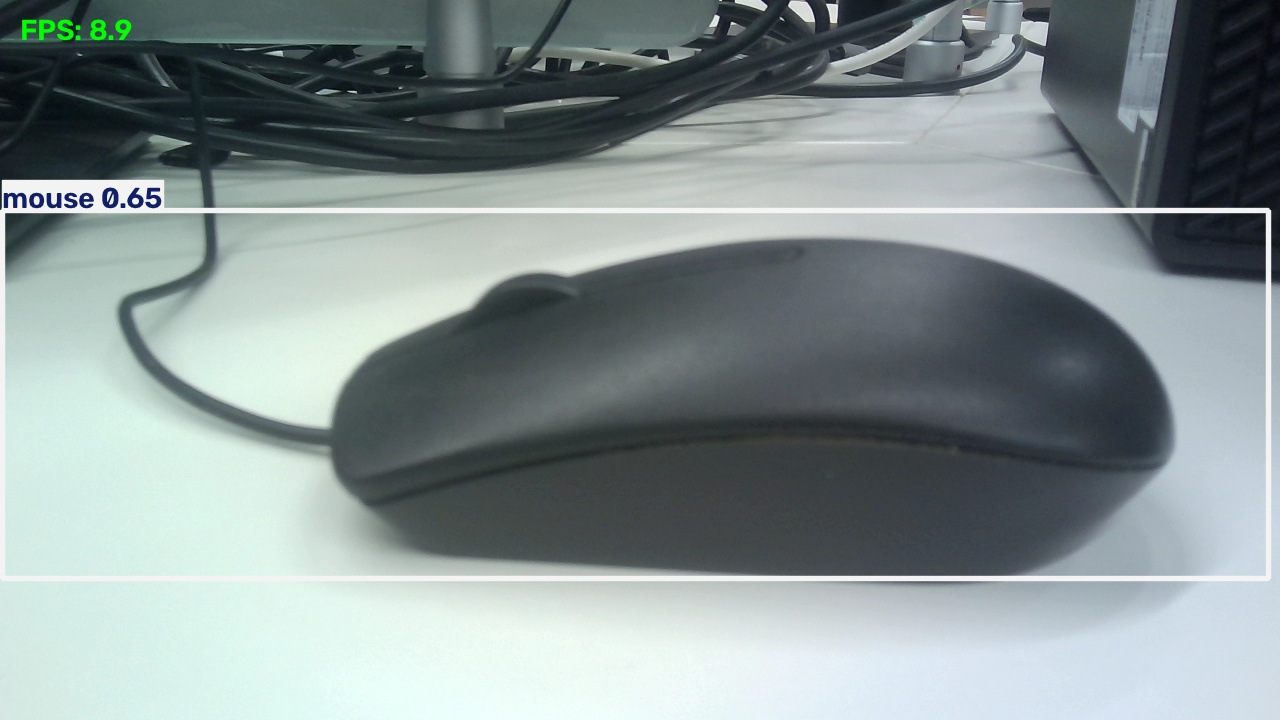
\includegraphics[width=0.82\textwidth]{report_assets/realtime_result_2.jpg}
\caption{Jetson 实时检测结果示例 2}
\label{fig:realtime2}
\end{figure}

\begin{figure}[H]
\centering
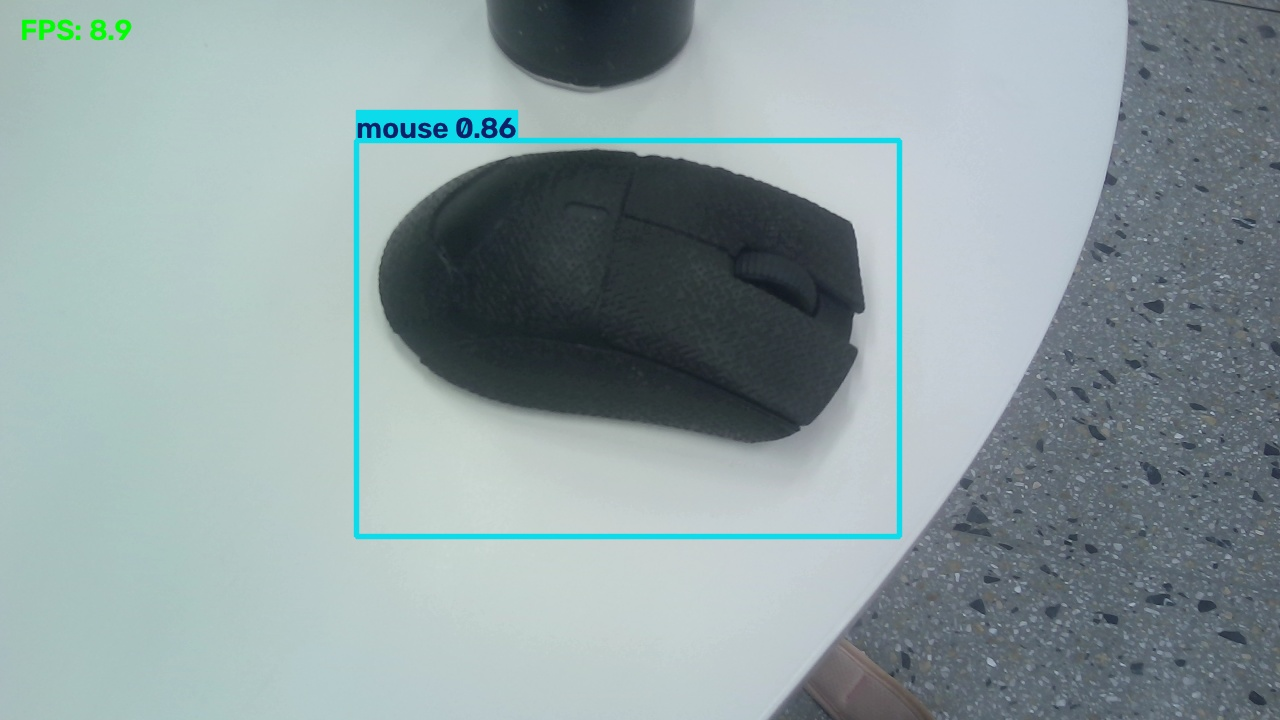
\includegraphics[width=0.82\textwidth]{report_assets/realtime_result_3.jpg}
\caption{Jetson 实时检测结果示例 3}
\label{fig:realtime3}
\end{figure}

\begin{figure}[H]
\centering
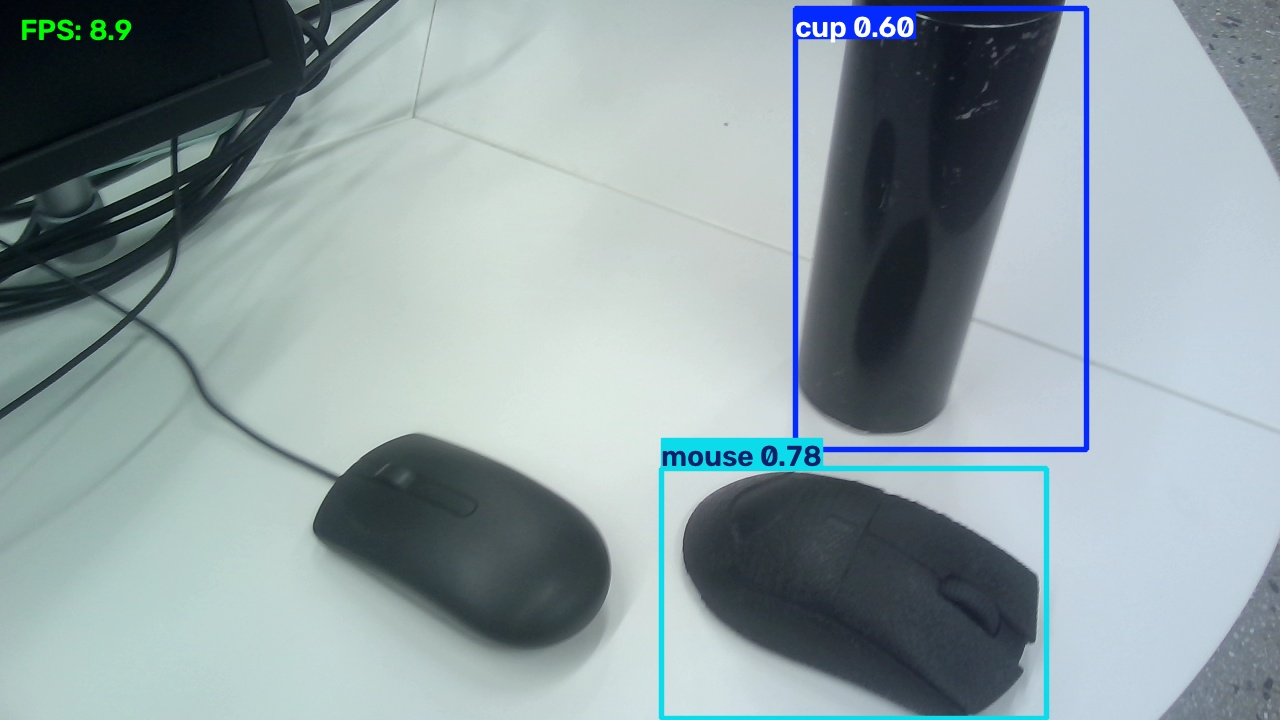
\includegraphics[width=0.82\textwidth]{report_assets/realtime_result_4.jpg}
\caption{Jetson 实时检测结果示例 4}
\label{fig:realtime4}
\end{figure}

\section{问题与优化}

实验过程中主要遇到以下问题：

\begin{enumerate}
  \item 在复杂背景中，模型可能将非目标物体误检为 cup 或 mouse；
  \item 当鼠标与人脸、手部或复杂背景重合时，目标边界不清晰，检测置信度会下降；
  \item ROS2 版本若同时发布原始图像和带框图像，会明显降低 Jetson 帧率；
  \item 直接使用较大输入尺寸会增加推理时间，影响实时性。
\end{enumerate}

对应优化方法如下：

\begin{enumerate}
  \item 增加真实桌面场景数据，尤其是负样本和容易误检的背景；
  \item 使用合适的置信度阈值，降低低置信度误检；
  \item 在 Jetson 上将输入尺寸调整为 \texttt{imgsz=320}，摄像头分辨率设置为 \texttt{640x480}；
  \item ROS2 版本默认只发布检测结果 topic，避免每帧发布大图像造成性能下降；
  \item 开启 Jetson 性能模式，提高实时推理速度。
\end{enumerate}

\section{实验结论}

本实验完成了从数据集构建、YOLO 模型训练、模型评估到 Jetson 实时部署的完整流程。最终 YOLOv8s v4 模型在测试集上取得了 mAP50 为 0.960 的结果，并能够在 Jetson 上进行实时 cup 和 mouse 检测。通过新增 ROS2 实时检测节点，模型检测结果被发布为 \texttt{/yolo/detections} topic，从而使目标检测模块具备接入机器人系统的能力。实验表明，将 YOLO 与 ROS2 结合部署到 Jetson 平台是可行的，可以作为后续机器人感知、目标定位和机械臂抓取任务的基础。

\end{document}
